\item \textbf{Intro}
\begin{itemize}
\item Draw a picture to show that conditioning creates a new random variable with a new distribution. Below, Figure 9 of note 26 does so by defining a random variable $\E(Y | X)$, which is a function of $X$. $\E(Y | X)$ is a random variable because giving $\E(Y | X)$ an outcome makes $X$ return a number, from which $\E(Y | X)$ (which is a number) can be calculated. 
I.e. $\E(Y | X)$ is a composition of a function on $X$ and a function on the outcome space.
I.e. $\E(Y | X)$ : $Ω \rightarrow R$
\begin{center}
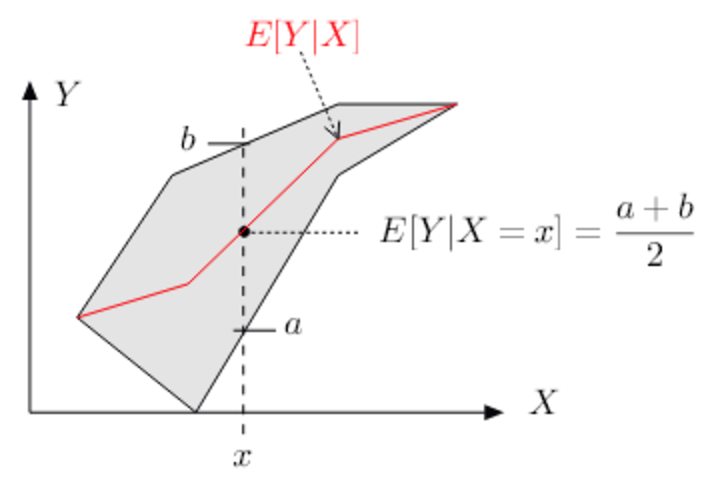
\includegraphics[width=8cm]{intro.jpg}
\end{center}
\end{itemize}